\documentclass{uai2025} % for initial submission
%\documentclass[accepted]{uai2025} % after acceptance, for a revised version; 
% also before submission to see how the non-anonymous paper would look like 
                        
%% There is a class option to choose the math font
% \documentclass[mathfont=ptmx]{uai2025} % ptmx math instead of Computer
                                         % Modern (has noticeable issues)
% \documentclass[mathfont=newtx]{uai2025} % newtx fonts (improves upon
                                          % ptmx; less tested, no support)
% NOTE: Only keep *one* line above as appropriate, as it will be replaced
%       automatically for papers to be published. Do not make any other
%       change above this note for an accepted version.

%% Choose your variant of English; be consistent
\usepackage[american]{babel}
% \usepackage[british]{babel}

%% Some suggested packages, as needed:
\usepackage{natbib} % has a nice set of citation styles and commands
    \bibliographystyle{plainnat}
    \renewcommand{\bibsection}{\subsubsection*{References}}
\usepackage{mathtools} % amsmath with fixes and additions
% \usepackage{siunitx} % for proper typesetting of numbers and units
\usepackage{booktabs} % commands to create good-looking tables
\usepackage{tikz} % nice language for creating drawings and diagrams

\usepackage{amsmath}
\usepackage{amssymb}
\usepackage{amsthm}
\usepackage{todonotes}
\usepackage{bm}
\usepackage{subcaption}
\usepackage[linesnumbered, ruled]{algorithm2e}

\def\ci{\perp\!\!\!\!\perp}

\newtheorem{definition}{Definition}
\newtheorem{proposition}{Proposition}
\newtheorem{theorem}{Theorem}

\title{Expert-In-The-Loop Causal Discovery: \\ Iterative Model Refinement Using Expert Knowledge}

% The standard author block has changed for UAI 2025 to provide
% more space for long author lists and allow for complex affiliations
%
% All author information is authomatically removed by the class for the
% anonymous submission version of your paper, so you can already add your
% information below.
%
% Add authors
\author[1]{\href{mailto:<ankur.ankan@ru.nl>?Subject=Your UAI 2025 paper}{Ankur~Ankan}{}}
\author[1]{Johannes~Textor}

% Add affiliations after the authors
\affil[1]{%
    Institute for Computing and Information Sciences\\
    Radboud University\\
    Nijmegen, The Netherlands
}
\begin{document}

\maketitle

\begin{abstract}
	Numerous causal discovery algorithms were developed to automatically learn
	directed acyclic graphs (DAGs) and other causal models from data. However,
	their adoption in applied domains remains limited, as researchers often
	prefer to construct DAGs manually based on domain knowledge. This
	preference arises due to several practical challenges with automated
	algorithms, such as their tendency to produce results that contradict
	obvious domain knowledge and their inability to distinguish Markov equivalent
	models. To assist researchers in constructing DAGs manually, we propose an iterative
	structure learning approach that combines domain knowledge with
	data-driven insights. Our method leverages conditional independence
	testing to iteratively identify variable pairs where an edge is
	either missing or superfluous. Based on this information, we can choose
	to add missing edges with appropriate orientation based on domain
	knowledge or remove unnecessary ones. We also give a method to rank
	these missing edges based on their impact on the overall model fit.
	In a simulation study, we find that this iterative approach to leverage domain 
	knowledge already starts outperforming purely data-driven structure learning if 
	the orientation of new edge is correctly determined in at least two out of three cases.
	We present a proof-of-concept implementation using a large language 
	model as a domain expert and a graphical user interface designed to 
	assist human experts with DAG construction.
\end{abstract}

\section{Introduction}
Understanding cause-and-effect relationships between variables is a fundamental
objective in many scientific fields. These relationships reveal the mechanisms
behind observed phenomena and guide effective interventions or policy
decisions. Causal discovery methods aim to discover such relationships among
random variables using observational data. In the DAG literature, the primary
focus has been on developing automated algorithms to learn causal structures
from datasets. These efforts have led to numerous causal discovery algorithms,
such as constraint-based methods like PC algorithm \citep{Spirtes2001,KalischB07} 
and Fast Causal Inference \citep{Spirtes2000}), score-based methods such as Hill-Climb
Search and Greedy Equivalence Search \citep{Chickering2002}, and continuous
optimization-based methods like NOTEARS \citep{Zheng2018} and DAGMA
\citep{Bello2022}. Despite significant progress in automated causal discovery,
their adoption in applied research has been limited. Challenges encountered with existing
causal discovery algorithms in practice include but are not limited to:

\begin{enumerate}
	\item \textbf{Lack of Trust:} While constraint-based algorithms are 
		often asymptotically
		consistent \citep{KalischB07}, they can and do make mistakes
		on  finite samples. These mistakes can be severe and contradict
		obvious domain knowledge (think of edges going into unmodifiable
		attributes such as Age). The choice of algorithm and hyperparameters
		significantly affects the output, making it
		difficult to assess reliability. Additionally, the absence of
		robust performance evaluation methods for any given dataset
		further reduce the confidence in their outputs. A recent paper
		therefore advised Epidemiologists to not attempt using structure
		learning algorithms without help of an expert \citep{Gururaghavendran_2024}.
	\item \textbf{Outputs Markov Equivalence Class (MEC):} As multiple
		DAGs can be faithful to a given observational dataset, automated 
		algorithms can only recover the MECs. These MECs can contain a
		combination of directed and undirected edges. This structural uncertainty
		can make it difficult or impossible to apply the learned model for downstream
		tasks, such as identification or causal
		effect estimation \citep{Maathuis_2009,PerkovicTKM17}.
\end{enumerate}

Figure~\ref{fig:intro} highlights some of these issues. In practice, DAGs 
are still largely constructed from domain knowledge alone 
\citep{Tennant2020,Petersen2021}. This can, however, be equally problematic.
Constructing DAGs requires us to distinguish between different causal structures, 
such as direct or indirect effects or causal mediation. Specifically, there is often a lack
of theoretical support for the \emph{absence} of direct causal effects, which are 
the key assumptions that graphical models make to enable downstream causal inferences.
Given the likelihood of making mistakes, it is therefore
important to at least validate the consistency of a DAG against our dataset. One way to
test this consistency is by testing whether the conditional independence 
(CI) statements implied by the DAG hold in the data \citep{Ankan2021}. Specifically, 
each missing edge between
a pair of variables in the DAG leads to one or more CI statements, 
which can be checked using statistical tests. Violations to CI
statements can point to the erroneous omission of important causal effects from a model
or to the presence of latent confounders.

% While DAG-based methods focus on
% automated discovery, SEM-based methods emphasize expert driven model
% specification. This includes tools to assist researchers in manually
% constructing models, enabling them to incorporate their domain knowledge in the
% model building process. Researchers typically begin with an initial model based
% on their domain knowledge and then use these tools to guide modifications that
% improve the model's fit to data. This process is commonly known as
% Specification Search \citep{Long1983} and uses method such as modification
% indices, and Wald-based tests \citep{Marcoulides2018}. 

\begin{figure}[t!]
    \begin{subfigure}{0.5 \textwidth}
	\centering
    	\includegraphics[page=1]{figures_v2.pdf}
    	\caption{}
    \end{subfigure}
    \begin{subfigure}{0.5\textwidth}
	\centering
    	\includegraphics[page=2]{figures_v2.pdf}
    	\caption{}
    \end{subfigure}
    \begin{subfigure}{0.5\textwidth}
	\centering
    	\includegraphics[page=3]{figures_v2.pdf}
    	\caption{}
    \end{subfigure}

    \caption{A comparison of Markov Equivalence Classes (MECs) learned from the Adult
	     Income Dataset \citep{Becker1996} using different causal discovery
	     algorithms and sample sizes. Edge colors represent the sample size
	     used: red for $N=400$, and blue for $N=800$. (a) PC algorithm with a
	     mutual information based CI test, (b) PC algorithm with a
    	     residualization-based test \citep{Ankan2023}, (c) Hill Climb Search with
	     Bayesian Information Criterion (BIC) score. The learned model structure varies
             significantly across different algorithms and sample sizes.}
    \label{fig:intro}
\end{figure}

In this paper, we propose a structure learning method that leverages this CI
testing approach to assist researchers during manual DAG construction, rather
than just validating the model. Our approach follows an iterative
model-building strategy that integrates domain expertise with CI testing on
data. At each iteration, we use CI testing to identify pairs of variables that
lack (direct or indirect) connections or are connected by a superfluous edge.
 We then use this information
along with domain expertise to determine which changes to make.
The orientation of the edge when adding is determined based on the domain
expertise; critically, this does not require the domain expert to distinguish 
between direct and indirect effects. Our resulting approach can be 
thought of as a guidance during manual model construction that ensures the 
model remains consistent to the data.

Our contributions are organized as follows:

\begin{enumerate}
    \item In Section~\ref{sec:modification}, we present our iterative method for DAG construction
	based on domain knowledge and data, and prove its correctness in an ``oracle setting''.
    \item We then present a ranking method to prioritize potential modifications to the DAG that 
    	    help in fixing the most severe violations first (Section~\ref{sec:ranking}).
    \item We show empirically that even experts that make mistakes can outperform purely 
	data-driven
	causal discovery algorithms (Section~\ref{sec:empirical}).
    \item We provide two proof-of-concept implementations of our approach: one geared towards
	LLMs as experts, and a graphical user interface designed 
	for human experts (Section~\ref{sec:web}).
\end{enumerate}

\section{Background}
\label{sec:background}
We denote random variables using uppercase letters like $X$, and a set of
random variables by $ \bm{X} = \{X_1, \cdots, X_k\} $, where $ \rvert \bm{X}
\rvert = k $ is the number of variables in the set. We denote the
covariance between variables $ X $ and $ Y $ as $ \mathrm{cov}(X, Y) $, a 
covariance matrix as $ \Sigma $, and the entry corresponding to the covariance
between $ X $ and $ Y $ as $ \Sigma_{XY} $. We consider causal DAGs that contain 
only observed variables. A DAG $ G = (V, E) $ is an acyclic directed graph
whose nodes $ V $ corresponding to random variables and whose edges $ E $ represent
direct causal relationships \cite{Pearl2009}. For an edge $e=X \to Y$, 
$\textrm{reverse}(e)=Y \to X$. The set of parents of $ X $ in $ G $
is denoted as $ \textrm{Pa}_G(X) $, and its ancestors and descendants as $
\textrm{An}_G(X) $ and $ \textrm{De}_G(X) $, respectively; we use the convention
that $X \notin \textrm{An}_G(X)$ and $X \notin \textrm{De}_G(X)$. We denote a path, $
\pi(X, Y) = \{ X, V_0, V_1, \cdots, V_k, Y \} $ between $ X $ and $ Y $ in $ G
$ where consecutive pairs of variables in $ \pi $ are connected by an
edge. We say $ X $ and $ Y $ are d-connected in $ G $ given a conditioning set
$ \bm{Z} \subseteq V - \{X, Y\} $, if for a path $ \pi(X, Y) $ (i) for every
collider structure ($ V_1 \rightarrow V_2 \leftarrow V_3 $) on $ \pi(X, Y) $, $
\bm{Z} \cap \{ V_2, \textrm{De}_G(V_2) \} \ne \emptyset $, and (ii) for every
non-collider structure ($ V_1 \rightarrow V_2 \rightarrow V_3 $, $ V_1
\leftarrow V_2 \rightarrow V_3 $), $ V_2 \not \in \bm{Z} $. $ X $ and $ Y $ are
\emph{d-separated} given $ \bm{Z} $ if no d-connecting path exist between them.

\subsection{Conditional Independence Tests}
\label{sec:ci_tests}
Our structure learning algorithm uses the idea of testing DAGs using CI statements
like $ X \ci Y \rvert \bm{Z} $ (with
potentially $ \bm{Z} = \emptyset $).
For example, take the MEC learned by the PC algorithm in
Figure~\ref{fig:intro}(b) using $ N=800 $, and suppose that we orient 
the undirected edge between \emph{Marital Status} and
\emph{Relationship}  as \emph{Marital Status} $ \rightarrow $
\emph{Relationship}. We can then read implied CIs of the DAG using $d$-separation,
and test them in our dataset. Figure~\ref{fig:ci_table} shows the result of some tests. 
Using a significance threshold  $\alpha=0.05 $, the first $ 2 $
implied CIs hold in the data whereas the remaining tests fail. One of the ways
to fix these failing tests is to add an edge between the variable pair $ X $
and $ Y $. While this method helps us in finding variable pairs where we need
to add an edge, it does not give us any information about the orientation of
this edge. In this paper, we use domain knowledge to determine this
orientation.

\begin{figure}
	\centering
	\begin{tabular}{llrr}
		$X$ & $Y$ & $ \bm{Z} $ & p-value \\
		\hline
		Incm & MrtS &  Age, Occp, Rltn & $ 0.29 $     \\
		Incm & Sex  &  Occp, Rltn      & $ 0.21 $     \\
		Incm & Wrkc &  Occp 	       & $ 1.5e^{-3} $ \\
		Edct & MrtS & Incm, Occp, Rltn & $ 0.02 $       \\
		\hline
	\end{tabular}
	\caption{Results of testing some of implied CIs of the DAG in
		 Figure~\ref{fig:intro}(b) using the same CI test that was used for
		 learning it.}
	\label{fig:ci_table}
\end{figure}

In addition to determining sigificance, we are interested in quantifying the 
\emph{strength} of any partial association between $X$ and $Y$ after conditioning 
on $\mathbf{Z}$. This metric depends on the type of CI test used. In the following,
we briefly overview some CI tests and effect size measures
for different types of (possibly mixed) data.

\paragraph{Both $ X $ and $ Y $ are continuous: }
When both $ X $ and $ Y $ are continuous, we can use a (partial) correlation
test for CI testing and Pearson's correlation coefficient can be used as the
effect size. When $ \bm{Z} = \emptyset $, the correlation coefficient is
defined as: $ r_{X, Y} = \mathrm{cov}(X, Y) / (\sigma_X \sigma_Y) $. When $
\bm{Z} \neq \emptyset $, the partial correlation coefficient can be used instead.
This is estimated by fitting two regression models $ E_X: X \sim \bm{Z} $ and $ E_Y: Y
\sim \bm{Z} $, calculating the residuals $ R_X = X - E_X(\bm{Z}) $ and $ R_Y =
Y - E_Y(\bm{Y}) $, and then computing the correlation coefficient between the
residuals: $r_{X, Y \rvert \bm{Z}} = r_{R_X, R_Y}$

\paragraph{$ X $ is ordinal, and $ Y $ and $ \bm{Z} $  are continuous or ordinal: }

Polyserial (for continuous $Y$) and polychoric
(ordinal $Y$) correlations are used to estimate correlations 
involving ordinal variables \citep{Poon1987}. Both methods make the assumption that the
observed ordinal variable is a result of thresholding a latent normally
distributed continuous variable. Under this assumption, the methods then 
estimate the threshold values and covariance matrix using maximum likelihood.
Using the estimated covariance matrix, $ \Sigma $ we can perform a correlation
test for CI and compute the Pearson's correlation coefficient as the effect
size in the same way as for continuous $ X, Y $ and $ \bm{Z} $, i.e., 
$\bm{Z} = \emptyset $, $ r_{X, Y} = \Sigma_{XY} / (\sqrt{\Sigma_{XX} \Sigma_{YY}}) $, 
	and when $ \bm{Z} \ne \emptyset $,
	$ r_{X, Y \rvert \bm{Z}} = - \Sigma^{-1}_{XY}/ (\sqrt{\Sigma^{-1}_{XX} \Sigma^{-1}_{YY}}) $.

\paragraph{$ X $, $ Y $, and $ \bm{Z} $ are all discrete (ordinal or categorical): }

For combinations of ordinal and categorical variables, we
can use a residualization-based CI test \citep{Ankan2023} that returns a 
chi-square distributed test statistic. Given the statistic, $ \chi^2 $, with $ \textrm{df} $ degrees of
freedom, we use the Root Mean Squared Error of Approximation (RMSEA) defined as
 $ \textrm{RMSEA}_{X, Y \rvert \bm{Z}} =
\sqrt{\max(0,\chi^2 - \textrm{df})/ (\textrm{df} (N-1))} $, where $ N $ is the sample
size. This effect size can be used for any statistical test with a chi-square 
distributed test statistic. 

\section{Expert-In-The-Loop Causal Discovery}


Our approach to causal structure learning combines domain knowledge with data-driven
insights in a manner that is based on the following considerations: 
(1) A domain experts is possibly good at determining causal directions between variables if 
there is a clear causal direction between them. (2) A domain expert may be less good
at identifying cases where there is no causal relationship between the variables,
since \emph{potential} causal relationships can often be argued for anyway.
(3) Many domain experts could struggle to distinguish direct from indirect 
effects, since the presence of a direct effect between two variables
of interest depends on all other variables present in the graph. 

We will now first present theoretical results showing how a structure
learning algorithm using such experts can uncover the true DAG structure.
Afterwards, we will present a heuristic for deciding which changes should
be prioritized.

\subsection{DAG Structure Learning using Ancestral Oracles}

\label{sec:modification}

We therefore consider the following two models of a domain experts: Given two variables
$ X $ and $ Y $ that are part of an unknown causal DAG $G$, an \emph{strong ancestral oracle} 
$\mathcal{A}_G$ is defined as:
$$\mathcal{A}_G(X,Y)=\begin{cases}
 X \to Y & \textrm{if } X \in \textrm{An}_G(Y) \\
 X \gets Y & \textrm{if } Y \in \textrm{An}_G(X) \\
 \textrm{None} & \textrm{otherwise} \\
\end{cases}$$

whereas a \emph{weak ancestral oracle} is defined as:
$$
\mathcal{A}_G(X,Y)=\begin{cases}
 X \to Y & \textrm{if } X \in \textrm{An}_G(Y) \\
 X \gets Y & \textrm{if } Y \in \textrm{An}_G(X) \\
 \textrm{rand}(X \gets Y, X \to Y) & \textrm{otherwise} \\
\end{cases}
$$

That is, our ancestral oracles only provide information on the direction of cause-effect
relationships, and do not distinguish between direct and indirect effects. 
The weak ancestral oracle is even unable to detect cases where there is no cause-effect
relationship between two variables. Using such oracles for DAG construction therefore 
inherently risks that superfluous edges are created. In our approach, such superfluous edges
will be detected and removed by utilizing the data. 

To model how our learning procedure interacts with the data, we assume that we
additionally have access to a second oracle $\mathcal{D}_G$ than can answer d-separation
queries with respect to the unknown target graph:
$\mathcal{D}_G(X,Y,\mathbf{Z})=1$ iff $X$ and $Y$ are $d$-separated by $\mathbf{Z}$ in 
$G$. These are the standard oracles considered in constraint-based structure learning
algorithms, such as the PC algorithm \cite{Spirtes2001}. 

Based on these two oracles, we now define two core procedures that we will use to 
iteratively change a current DAG structure. The procedure 
\textsc{Expand} (Algorithm~\ref{algo:expand}) uses conditional independence
information to search for missing edges in the graph and then uses domain
knowledge to orient them. The procedure \textsc{Prune} (Algorithm~\ref{algo:prune}) uses
conditional independence information to remove superfluous edges from the
graph.

\begin{algorithm}[h]
\DontPrintSemicolon
\SetAlgoLined
\SetKwFunction{Expand}{Expand}
\SetKw{KwGoTo}{go to}
\SetKwProg{Fn}{Function}{:}{}
\Fn{{\sc Expand}($V,E,\mathcal{D}_G,\mathcal{A}_G$,$B$,$k$)}{
    let $L \gets \{\}$\;
    \ForEach{$X, Y$ where $X \to Y \notin E$ and $Y \to X \notin E$ and 
	$\{X,Y\} \notin B$}{
        let $\mathbf{Z}$ be a set that $d$-separates $X$ and $Y$ in $(V,E)$\;
        \If{$\mathcal{D}_G(X, Y, \mathbf{Z}) = 0$}{
	    $e \gets \mathcal{A}_G(X, Y)$ \;
	    \uIf{ $(V,E \cup L \cup e)$ is acyclic }{
            	$L \gets L \cup  \{ e \} $\;
	    } \Else {
            	$L \gets L \cup  \{ \textrm{reverse}(e) \} $\;
	    }
        }
	\If{$|L|\geq k$}{\KwGoTo 12\;}
    }
    add all edges in $L$ to $E$\;
    \Return{$(V,E)$}\;
}
\caption{Adding edges based on data and domain knowledge.}
\label{algo:expand}
\end{algorithm}

The function $\textsc{Expand}$ takes an initial list of edges and searches for 
any vertex pairs that are not connected but where the d-separation oracle 
indicates  that there is still a residual association not explained by the other variables.
An optional parameter $B$, the empty set by default, allows to specify a ``black list''
of vertex pairs that must not be connected, and another optional parameter $k$
specifies the maximum amount of edges to be added by this procedure.

Let $G^+$ denote the transitive closure of $G$, that is, the graph in which 
there is a direct edge $X \to Y$ whenever $X \in \textrm{An}_G(Y)$. The transitive
closure is related to the result of $\textsc{Expand}$ by the following two 
easily proved facts.

\begin{proposition}
For a conditional independence oracle
 $\mathcal{D}_G$ and a strong ancestral oracle $\mathcal{A}_G$, 
$\textsc{Expand}(V,\emptyset,\mathcal{D}_G,\mathcal{A}_G, \emptyset, \infty)=G^+$.
\label{prop:strongexpand}
\end{proposition}

\begin{proof}
Since we start from an empty graph, every pair of vertices $X, Y$ where
 $X \in \textrm{An}_G(Y)$ is d-separated by the empty set and is
 connected by the edge $X \to Y$. No other edges are added. Therefore, 
the result is $G^+$. 
\end{proof}

\begin{proposition}
For a conditional independence oracle
 $\mathcal{D}_G$ and a weak ancestral oracle $\mathcal{A}_G$, 
$\textsc{Expand}(V,\emptyset,\mathcal{D}_G,\mathcal{A}_G, \emptyset, \infty)
\supseteq G^+$.
\label{prop:weakexpand}
\end{proposition}

\begin{proof}
Every pair of vertices $X, Y$ that are $d$-connected in $G$ are now connected by an edge 
during $\textsc{Expand}$. For $X \in \textrm{An}_G(Y)$, the edge is 
$X \to Y$ just like when using a strong ancestral oracle; since only correctly oriented
edges are added between ancestor-descendant pairs, such additions never create cycles.
For $X, Y$ that are only $d$-connected throug common ancestors, an arbitrary 
edge is added in a manner that preserves acyclicity. The result is a supergraph
of $G^+$.
\end{proof}


\begin{algorithm}[h]
\DontPrintSemicolon
\SetAlgoLined

\SetKwProg{Fn}{Function}{:}{}
\Fn{{\sc Prune}($V$,$E$,$\mathcal{D}_G$)}{
    let $L \gets \{\}$\;
    \ForEach{$X \to Y \in E$}{
        remove $X \to Y$ from $E$\;
        let $\mathbf{Z}$ be a set that $d$-separates $X$ and $Y$ in $(V,E)$\;
        \If{$\mathcal{D}_G(X, Y, \mathbf{Z}) = 1$}{
            $L \gets L \cup  \{X \to Y\}$ \;
        }
    }
    remove all edges in $L$ from $G$\;
    \Return{$(V,E)$}\;
}
\caption{Pruning superfluous edges}
\label{algo:prune}
\end{algorithm}

Unlike our ancestral oracles, the pruning operation is quite effective at distinguishing
direct and indirect effects, as shown by the following result.

\begin{proposition}
Consider two DAGs $G=(V,E)$ and $G'=(V,E')$ where $E \subseteq E'$. 
Then $\textsc{Prune}(G',\mathcal{D}_G)=G$.
\label{prop:prune}
\end{proposition}

\begin{proof}
For an edge $X \to Y$ in the skeleton of $G$, $\mathcal{D}_G(X, Y, \mathbf{Z}) = 0$ regardless 
of $\mathbf{Z}$, so all edges in the skeleton are retained after {\sc Prune}. Conversely, if 
 $X \to Y$ is not in the skeleton of $G$, let $\mathbf{Z}$ be the $d$-separating set chosen 
in line~5 of {\sc Prune} (there is at least one such $\mathbf{Z}$, the union of the parents of 
$X$ and $Y$). Since  $\mathbf{Z}$ $d$-separates all paths from $X$ to $Y$ in $G'$, it does the same 
in $G$ which contains a subset of these paths. Therefore, all edges not in the skeleton of $G$ are 
removed.
\end{proof}

By combining Propositions~\ref{prop:strongexpand}, \ref{prop:weakexpand} and 
\ref{prop:prune}, we immediately obtain the following:

\begin{theorem}
Given a d-separation oracle $\mathcal{D}_G$ and a strong or weak 
ancestral oracle $\mathcal{A}_G$, 
$\textsc{Prune}(\textsc{Expand}((V,\emptyset),\mathcal{D}_G,\mathcal{A}_G,\emptyset,\infty),\mathcal{D}_G)=G.$
\end{theorem}

Since we require expert knowledge only in the $\textsc{Expand}$ operation, we may try
to be more economical by asking fewer questions at a time and interleaving expansion and
pruning steps. This leads us to the following, more incremental DAG construction algorithm.

\begin{algorithm}[h]
\DontPrintSemicolon
\SetAlgoLined
\SetKwProg{Fn}{Function}{:}{}

\Fn{{\sc ExpertInLoop}($V,\mathcal{D}_G,\mathcal{A}_G$)}{
$E_p \gets \emptyset$ \tcc{Current edges} 
$B \gets \emptyset$ \tcc{Edges that were pruned} 
\Repeat{ $E=E_p$ }{
	$E \gets E_p$ \;
	$(V,E) \gets \textsc{Expand}(V,E,\mathcal{D}_G,\mathcal{A}_G,B,1)$ \;
	$(V,E_p) \gets \textsc{Prune}(V,E,\mathcal{D}_G)$ \;
	$B \gets B \cup \{ E_p \setminus E \} $
}
\Return{(V,E)}
}

\caption{Iterative structure learning with expert in the loop}
\label{algo:expert}
\end{algorithm} 

\begin{theorem}
Let $G=(V,^*E)$ be a DAG, $\mathcal{D}_G$ a d-separation oracle for $G$, and 
$\mathcal{A}_G$ a strong or weak ancestral oracle for $G$. Then 
$\textsc{ExpertInLoop}(V,\mathcal{D}_G,\mathcal{A}_G)=G$.
\end{theorem}

\begin{proof}
The loop in Algorithm~\ref{algo:expert} terminates if and only if $E=E^*$. If the loop does not 
terminate, a new edge has been added in line 6, and/or one or more edges were pruned in line 7; the pruned 
edges never include the edge added in line 6 in the same iteration.
Every edge can be added at 
most once and pruned at most once. Therefore, the algorithm always terminates
after at most $|V|(|V|-1)+1$ iterations of the loop. For every edge $e=X\to Y $ in the skeleton of $G$, $\mathcal{D}_G(X,Y,\mathbf{Z})=0$ irrespective of $\mathbf{Z}$, and $e$ must be added to $E$ in some iteration, and can never be pruned afterwards. Therefore, after some iteration, $(V,E)$ must be a supergraph of $G$ after executing line 6, and this will be pruned to the real graph $G$ in line 7 (Proposition~\ref{prop:prune}). In the next iteration, no further changes are made, and the loop terminates.
\end{proof} 


\begin{figure}[t!]
	\begin{subfigure}{0.125 \textwidth}
		\centering
		\includegraphics[page=1]{example.pdf}
		\caption{True DAG}
	\end{subfigure}%
	\begin{subfigure}{0.125 \textwidth}
		\centering
		\includegraphics[page=2]{example.pdf}
		\caption{No edges.}
	\end{subfigure}%
	\begin{subfigure}{0.125 \textwidth}
		\centering
		\includegraphics[page=3]{example.pdf}
		\caption{$ X_1 \rightarrow X_4 $}
	\end{subfigure}%
	\begin{subfigure}{0.125 \textwidth}
		\centering
		\includegraphics[page=4]{example.pdf}
		\caption{$ X_1 \rightarrow X_2 $}
	\end{subfigure}
	\begin{subfigure}{0.125 \textwidth}
		\centering
		\includegraphics[page=5]{example.pdf}
		\caption{$ X_1 \rightarrow X_3 $}
	\end{subfigure}%
	\begin{subfigure}{0.125 \textwidth}
		\centering
		\includegraphics[page=6]{example.pdf}
		\caption{$ X_2 \rightarrow X_4 $}
	\end{subfigure}%
	\begin{subfigure}{0.250 \textwidth}
		\centering
		\includegraphics[page=7]{example.pdf}
		\caption{$ X_3 \rightarrow X_4 $. $ X_1 \not \rightarrow X_4 $.}
	\end{subfigure}
	\caption{An example showing each iteration of the \textsc{ExpertInLoop} algorithm. The dashed edges show all the potential edges that \textsc{Expand} step could add in each iteration.}
\end{figure}


\subsection{Ranking Potential New Edges}
\label{sec:ranking}

\begin{algorithm}[h]
\DontPrintSemicolon
\SetAlgoLined
\SetKwFunction{RankedExpand}{RankedExpand}
\SetKw{KwGoTo}{go to}
\SetKwProg{Fn}{Function}{:}{}
\Fn{{\sc RankedExpand}($V,E,\mathcal{D}_G,\mathcal{A}_G$,$\phi$,$B=\emptyset$)}{
    let $\phi_{\max} \gets 0 $\;
    \ForEach{$X, Y$ where $X \to Y \notin E$ and $Y \to X \notin E$ and 
	$\{X,Y\} \notin B$}{
        let $\mathbf{Z}$ be a set that $d$-separates $X$ and $Y$ in $(V,E)$\;
        \If{$\mathcal{D}_G(X, Y, \mathbf{Z}) = 0$}{
		\If{$\lvert \phi(X, Y, \mathbf{Z}) \rvert > \phi_{\max}$}{
			$ \phi_{\max} \gets \lvert \phi(X, Y, \mathbf{Z}) \rvert $ \;
			$ e_{\max} \gets \mathcal{A}_G(X, Y)$ \;
		}
        }
    }

    \uIf{ $(V,E \cup e_{\max})$ is acyclic }{
	add $ e_{\max}$ to $E$ \;
    } \Else {
	add $ \textrm{reverse}(e_{\max})$ to $E$ \;
    }
    \Return{$(V,E)$}\;
}
\caption{Adding an edge between variables with the highest correlation}
\label{algo:ranked_expand}
\end{algorithm}

The \textsc{ExpertInLoop} algorithm adds a new edge in each iteration. The edge
to be added is selected using the \textsc{Expand} algorithm, which returns a
potential edge at random based on the iteration order. However, if the residual
association between the selected variables is low, adding the edge may result
in only a marginal improvement in the overall model fit. Given that the
algorithm requires expert intervention in each iteration to specify the edge
orientation, it is beneficial to prioritize edges that contribute the most to
improving the model.

To achieve this, instead of selecting edges randomly, we propose ranking
potential edges based on their residual association given the current DAG. This
residual association can be quantified using the effect size measures from the
CI tests used for querying the d-separation in Algorithm~\ref{algo:expand}.
Specifically, for a d-separation query $ D_G(X, Y, \mathbf{Z}) $, we quantify
the residual association, $ \phi(X, Y, \bm{Z}) $, as the effect size of the CI
test $ X \ci Y \rvert \bm{Z} $. In Algorithm~\ref{algo:ranked_expand}, we
outline a greedy approach to edge selection using the effect size measure. 

To implement Algorithm~\ref{algo:ranked_expand}, we need to have an effect size
metric by which we can rank effects. Depending on the type of variables, we can
use the effect size measures shown in Section~\ref{sec:ci_tests}. The algorithm
selects the edge that has the highest absolute residual association, resulting
in prioritization of edges that contribute the most to improving the model.

\subsection{Connection to Score-Based Methods}

Our procedure shares similarities with score-based automated causal discovery
methods, such as Greedy Equivalence Search (GES), where the algorithm
iteratively adds or removes edges that maximize improvements in a specified
scoring metric. Given a scoring metric, --total residual association, $ \tau $ for 
a DAG $ G = (V, E) $, defined as:

\begin{equation}
	\tau = \sum_{\substack{X, Y \in V \\ X \rightarrow Y, Y \rightarrow X \not \in E}}   \phi(X, Y, \mathrm{pa}_G(X) \cup \mathrm{pa}_G(Y))
\end{equation}

our \textsc{RankedExpand} approach behaves similarly to GES. In each iteration,
we add the edge between the variable pair that results in the lowest $ \tau $
and remove edges that have no impact on $ \tau $.

While both methods aim to make iterative modifications to the DAG, a key
distinction lies in the nature of the evaluation criteria: unlike standard
scoring metrics, $ \tau $ is not decomposable. Decomposibility is a key
property of scoring metrics, allowing them to be expressed as the sum of
individual variables in the model. This property ensures that adding or
removing an edge only affects a localized part of the model. In contrast, $
\tau $ can not be decomposed, as modifying an edge in one part of the model can
affect the residual associations in other parts of the model.

Another key difference lies in the interpretability of the evaluation metric.
Scoring metrics are based on usually based on the log-likelihood with a penalty
for model complexity. They can be used to make relative comparisons between
models but their values do not have any interpretation in an absolute sense.
That is, they indicate which model is better for a given dataset but do not
quantify how well the model explains the data in an absolute sense. In
contrast, $ \tau $ provides an absolute measure of model fit -- its value
approaches $ 0 $ as the model perfectly explains the observed data.


\section{Empirical Analysis}
\label{sec:empirical}

In this section, we compare our \textsc{ExpertInLoop} algorithm with automated
causal discovery algorithms. Our goal with the empirical analysis is to
understand the behaviour of our method when the experts are not perfect. To
simulate this imperfect expert, we use a version of the strong ancestral oracle
that has an accuracy of $ \alpha $:

\begin{equation}
	\begin{split}
		x &= \textrm{rand}([0, 1]) \\
		\mathrm{Expert}(\alpha) &= \begin{cases} 
			\mathcal{O}(X, Y),  & \textrm{if  } x <= \alpha \\
			\textrm{rand}(X \rightarrow Y, Y \leftarrow X, \textrm{None}) & \textrm{otherwise} \\
				\end{cases} \\
			\mathcal{O}(X, Y) &= \begin{cases}
				X \rightarrow Y, & \textrm{if } X \rightarrow Y \in G_{\textrm{true}} \\
				Y \rightarrow X, & \textrm{if } Y \rightarrow X \in G_{\textrm{true}} \\
					\textrm{None}, & \textrm{otherwise }
				  \end{cases}
	\end{split}
\end{equation}

where $G_{\textrm{true}}$ is the true data generating DAG.

An important point to note here is that the effective accuracy of $
\mathrm{Expert} $ is higher than $ \alpha $ as even when giving a random
answer, there is a $ 1 $ in $ 3 $ chance that the answer is correct. Therefore,
an $ \mathrm{Expert} $ with accuracy $ \alpha $, has an effective accuracy, $ \alpha_{\mathrm{eff}} = \alpha + (1 - \alpha) / 3 $.

\begin{figure}[t!]
	\centering
	\begin{subfigure}{0.5\textwidth}
		\centering
		\includegraphics{../code/fig3/shd_ribbon.pdf}
		\caption{}
	\end{subfigure}
	\begin{subfigure}{0.5\textwidth}
		\centering
		\includegraphics{../code/fig3/sid_ribbon.pdf}
		\caption{}
	\end{subfigure}
	\caption{Comparison of PC, Hill-Climb Search, and GES algorithms against
		\textsc{ExpertInLoop} algorithm. As automated algorithms only
		recover the CPDAG, we use the best and worst scoring
		orientation of the CPDAG to get the range. We test
		\textsc{ExpertInLoop} with varying values of expert accuracy, $ \alpha = \{0.1, 0.3, 0.5, 0.7, 0.9\} $. The corresponding
		$\alpha_{\textrm{eff}} $ is shown in the plot.}
	\label{fig:shd_sid}
\end{figure}

We analyzed the performance of \textsc{ExpertInLoop} algorithm by comparing it
with three other automated algorithms: PC, Hill-Climb Search, and Greedy
Equivalence Search (GES) on linear Gaussian data. For \textsc{ExpertInLoop}, we
use the \textsc{RankedExpand} method with Pearson's correlation coefficient as
the effect size measure (Section~\ref{sec:ci_tests}). For the analysis, we
simulated data from known DAGs and use the algorithms to recover the original
DAG. We start by generating a random DAG on $10$ nodes and use linear models
with random effects to simulate $ 500 $ samples from it. We simulate each
variable $ V_i $ in the DAG as:


\begin{equation}
	\begin{split}
		\bm{\beta} &= \mathrm{Uniform}([-0.6, 0.6]) \\
		V_i &= \bm{\beta} \mathrm{Pa}_G(V_i) + \mathcal{N}(0, 1)
	\end{split}
\end{equation}

We perform the experiment for both varying densities of the DAG and accuracy of
$\mathrm{Expert}$. We also repeat each experiment $ 30 $ times and report the
mean and standard error of the results.

To compare the learned DAG to the original DAG, we use two metrics: Structural
Hamming Distance (SHD) and Structural Intervention Distance (SID)
\citep{Peters2015}. Unlike \textrm{ExpertInLoop}, the automated algorithms can
only recover the MEC, therefore, we considered all possible orientations of the
MEC to compute a range of SHD and SID values representing the best and worst
case scenarios. The results of this analysis are shown in
Figure~\ref{fig:shd_sid}. For SHD, the performance of \textsc{ExpertInLoop} is
comparable to the automated algorithms for $ \alpha = 0.3
(\alpha_{\textrm{eff}} = 0.53 $, implying that if an expert is able to get the
edge orientation correctly in more than $ 1 $ out of $ 2 $ cases, they can
outperform the automated algorithms. Similarly for SID, an expert can outperform 
the automated algorithms if they are able to get the orientation correct in $ 2 $ 
out of $ 3 $ cases. Another thing to note is that for denser DAGs, the 
\textsc{ExpertInLoop} is able to perform better for lower $ \alpha $ values.

\begin{figure}[t!]
	\begin{subfigure}{0.25\textwidth}
		\centering
		\includegraphics{../code/fig4/unexplained_effect.pdf}
		\caption{}
	\end{subfigure}%
	\begin{subfigure}{0.25\textwidth}
		\centering
		\includegraphics{../code/fig4/ll.pdf}
		\caption{}
	\end{subfigure}
	\caption{LLM-in-the-loop causal discovery on the Adult Income datases. As the ground 
truth is unknown, two measures of fit are shown over 30 iterative modifications: 
total residual association $\tau$ (a, lower is bettter); log-likelihood (a, higher is better).
	}
	\label{fig:unexplained_ll}
\end{figure}

\section{Practical Implementation}

\label{sec:web}

We now present two proof-of-concept implementations of our approach, 
geared towards using  large language models (LLMs) and humans as experts
to decide on edge directions. We use the Adult Income dataset from the 
introduction as an example. There is no known ground truth for this dataset,
and it contains mixed types of data; here, we use a version that contains
ordinal and nominal variables and use the RMSEA as a measure of association
to prioritize modifications (Section~\ref{sec:background}). 

\subsection{Using LLMs as Experts}
 
\begin{figure}[t!]
	\centering
	\includegraphics[page=1]{fig5.pdf}
	\caption{DAG learned from the Adult Income dataset using an LLM
		(Gemini 1.5 Flash) as the expert. The p-value threshold used is $ 0.05 $ 
		and the measure of association threshold is $ 0. 1 $}
	\label{fig:adult_llm}
\end{figure}

Recently, there has been significant interest in leveraging Large Language
Models (LLMs) for causal discovery. These applications range from determining
pairwise edge orientations \citep{Kiciman2023, Jin2024} to full causal
structure learning \citep{Naik2023, Vashishtha2023} and counterfactual
reasoning \citep{Kiciman2023} (see \citet{Liu2024} for a comprehensive
overview).

Since our approach relies on expert knowledge to determine edge orientations,
we explored the potential of using an LLM for this task. We applied our causal
discovery procedure using the Gemini 1.5 Flash model as the expert. We simulate
the \emph{weak ancestral oracle} using the LLM by asking it to choose the
causal direction between a pair of variables. The LLM is provided a description
of each of the variables and given the prompt shown in
Appendix~\ref{section:llms}. 
Figure~\ref{fig:unexplained_ll} shows how the model fit to the data improves 
across 30 iterations compared to GES for a run of the algorithm.
Figure~\ref{fig:adult_llm} shows the DAG learned
on the Adult Income dataset using the LLM as the expert. We can see 
that the model fit improves comparably to a greedy approach and 
the resulting DAG contains largely sensible edge directions. 

\subsection{Using Humans as Experts}


\begin{figure}[t!]
	\centering
	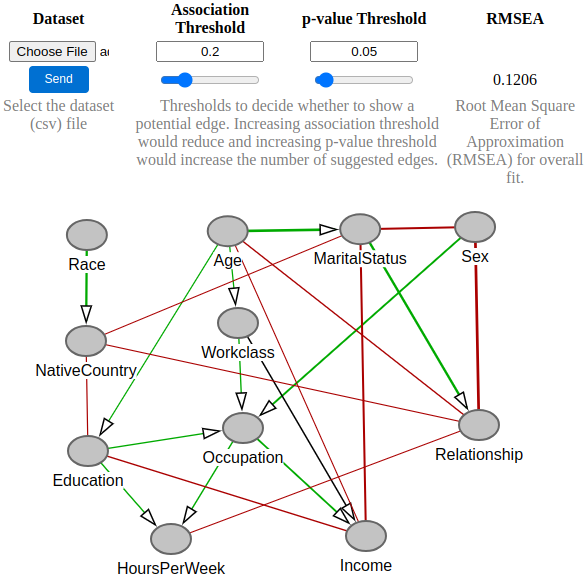
\includegraphics[scale=0.4]{../code/plots/web_tool_full_new.png}
	\caption{A screenshot of the web tool for constructing the model. Users
		can upload their dataset after which the tool creates an empty
		graph and shows all pair of variables which are associated in
		the model using undirected red edges with the strength of
		association represented using edge width. Users can then
		iteratively add edges to the model (shown in green) while
		deciding the edge orientation based on domain knowledge.
		Unnecessary edges are shown in black.}
	\label{fig:web}
\end{figure}

To enable researchers to easily apply our approach to their own datasets, we
developed an interactive web-based tool (Figure~\ref{fig:web}) for constructing
DAGs. Users can upload their dataset, which initializes an empty DAG with nodes
corresponding to the dataset's variables. They can then specify a p-value
threshold and a threshold for a minimal association strength. The tool 
then visually highlights variable pairs
with a residual association greater than the threshold, marking them with red
edges; to avoid cluttering, no lines are drawn for residual associations that
are statistically insignificanct or below the specified threshold.
The thickness of these edges represents the strength of association,
helping users prioritize which variable pairs to address first; however, note that
users are free to choose which variables to connect. Similarly, if
an existing edge is found to be potentially superfluous (statistically insignificant),
it is highlighted in black. Using this information, users can iteratively
modify the model by adding or removing edges. The tool also computes the Root
Mean Square Error of Approximation (RMSEA) based on Shipley's C test, a global test 
of model fit based on the implied CIs \citep{Shipley2000}, to provide an estimate of the
overall fit of the model. Once satisfied with the constructed DAG, users can
export the model for further analysis.

\section{Conclusions}

Researchers often prefer to construct DAGs manually rather than using automated
algorithms due to practical challenges in applying automated methods. To assist
this process, we developed an iterative structure learning method that
integrates manual construction with data-driven feedback, bridging
the gap between fully manually and fully automated methods.
The idea of augmenting structure learning by domain knowledge is of course not 
new. Common ways to provide such background knowledge are "whitelists" or "blacklists"
of edges that must or must not be present in the resulting DAG, or specification
of a temporal structure between the variables. 
Compared to such approaches, where domain knowledge 
is specified and supplied beforehand, the novelty of our method lies in the interactive
back-and-forth between domain knowledge and data, which provably leads to the correct
result in a polynomial amount of steps (if the expert answers all
ancestral queries correctly).

Avenues for future work include extending this approach to latent variables 
as encoded by acyclic directed mixed graphs (ADMGs). Further, if experts make 
mistakes that lead to inconsistencies during model construction (such as cycles),
this information could be leveraged in a more systematic way to allow backtracking
and recovery.

\begin{acknowledgements} 
	We acknowledge the use of ChatGPT (\url{https://chatgpt.com/}) for
	proofreading parts the manuscript.
\end{acknowledgements}

\bibliography{references}

\newpage

\onecolumn
\title{Expert-In-The-Loop Causal Discovery: Iterative Model Refinement Using Expert Knowledge \\ (Supplementary Material)}
\maketitle
\appendix

\section{Prompts Used for LLM}
\label{section:llms}

\begin{figure}[ht!]
	\centering
	\begin{verbatim}
You are an expert in Social Science. Following are the descriptions of two variables:

<A>: {description of variable A}
<B>: {description of variable B}

Which of the following two options is the most likely causal direction between these 
variables:

1. <A> causes <B>
2. <B> causes <A>

Return a single letter answer between the choices above; Do not provide any reasoning 
in the answer; Do not add any text formatting to the answer.
	\end{verbatim}
	\caption{Prompt used for the LLM. Here the variable descriptions are replaced with description provided in Fig.~\ref{fig:var_description}}
	\label{fig:prompt}
\end{figure}

\begin{figure}[ht!]
	\begin{verbatim}
          Age: The age of a person
    Workclass: The workplace where the person is employed such as Private industry, 
     	       or self employed
    Education: The highest level of education the person has finished.
MaritalStatus: The marital status of the person
   Occupation: The kind of job the person does. For example, sales, craft repair, 
   		clerical.
 Relationship: The relationship status of the person.
         Race: The ethnicity of the person.
          Sex: The sex or gender of the person.
 HoursPerWeek: The number of hours per week the person works.
NativeCountry: The native country of the person.
       Income: The income i.e. amount of money the person makes.
	\end{verbatim}
	\caption{Variable descriptions used for prompting the LLM}
	\label{fig:var_description}
\end{figure}

\section{A Generalized Measure of Conditional Association}
\label{sec:mixed_association}

In the previous section, we discussed how different types of variables require
different measures of conditional association. However, there is no unified
measure that handles mixed data. In this section, we introduce a measure of conditional
association for mixed data by extending the concept of partial correlation
coefficient (commonly used for continuous variables) to mixed data. Similar to
partial correlation coefficient, our method integrates a mixed data
residualization method \citep{Ankan2023} with Pillai's Trace
\citep{Pillai1955}, a multivariate measure of association based on canonical
correlations.
 
Given a dataset $ D = (x, y, \bm{z}) $ on variables $ X $, $ Y $, and $ \bm{Z}
$, our goal is to estimate the conditional association $ \phi_{X, Y; \bm{Z}} $. 
In the first step, we compute the residuals $ R_X $ and $ R_Y $ for variables
$ X $ and $ Y $ respectively. Depending on the type of variable the residual
is computed as follows:

\begin{enumerate}
	\item \textbf{Continuous:} We train a model, $ E_X: x \sim
		\bm{z} $. The residuals are then computed by taking the difference
		between the true and the predicted values using $ E_X $. 
		$$ R_{x_i} = x_i - E_X(\bm{z}_i) $$
	\item \textbf{Ordinal:} We start by training a probability estimator, $
		p_X: x \sim \bm{z} $, and then use the estimated probabilities, 
		$ \hat{p}_X(x) $ to compute the residuals:
		$$ R_{x_i} = \hat{p}_X(X < x_i) - \hat{p}_X(X > x_i) $$
	\item \textbf{Categorical:} We again start by training a probability
		estimator $ p_X: x \sim \bm{z} $, and obtain probability
		estimates $ \hat{p}_X: p_X(\bm{z}) $. Next, we dummy encode the
		categorical variable, resulting in a binary vector and then
		compute the residuals as follows: 
		$$ R_{x_i} = x_i - \hat{p}_X(\bm{z}_i) $$
\end{enumerate}

We have the option here to choose the estimators based on the characteristics
such as distribution, type of relationship, and so on of our dataset.
Non-parametric ensemble estimators such as Random Forest and XGBoost are robust 
for diverse data types and complex relationships. For linear relationships,
simpler models such as linear regression and its variants may suffice.

We repeat the above residualization step for both the variables $ X $ and $ Y $
obtaining residual matrices $ R_x $ and $ R_y $. The type of variable determines
the shape of these matrices. If the variable is continuous or ordinal, the 
residual matrix is of shape $ (n \times 1 ) $ and if the variable is categorical,
we get a residual matrix of shape $ (x \times (k - 1)) $, where $ k $ is the number
of categories of the variable.

The second step is to quantify the association between these residual matrices.
For this purpose we use canonical correlations \citep{Hotelling1936} that have been widely used to
measure the association between sets of random variables.

\begin{definition}
	Given two sets of random variables $ \bm{U} = (U_1, U_2, \cdots, U_p) $
	and $ \bm{V} = (V_1, V_2, \cdots, V_q) $, canonical correlation between
	them, $\rho_{\bm{U}, \bm{V}} $ is defined as:
		
	\begin{equation}
		% \nu_{\bm{U}, \bm{V}}= \max_{a, b} \mathrm{corr}(a^T \bm{U}, b^T \bm{V})
		\rho_{\bm{U}, \bm{V}} = \max_{a, b} \frac{a^T \Sigma_{\bm{UV}} b}{\sqrt{a^T \Sigma_{\bm{UU}} a \cdot b^T \Sigma_{\bm{VV}} b}}
	\end{equation}

	where $ a $ and $ b $ are vectors of coefficients that maximize the correlations
	between the linear combinations of $ a^T \bm{U} $ and $ b^T \bm{V} $.
\end{definition}

Canonical correlations generalize the concept of correlation coefficients to
multi-dimensional variables. It finds orthogonal linear transformations $ a $
and $ b $ that maximized the correlation between the transformed variables $
a^T \bm{U} $ and $ b^T \bm{V} $. This yields a vector of correlation
coefficient values of size $ \min(p, q) $, representing the correlation
coefficient of each pair of transformed variables. Notably, Pearson's
correlation coefficient is a special case of canonical correlations when $ p =
q = 1 $.

Several measures of association have been derived from canonical correlations, such as:
\begin{itemize}
	\item Wilks' Lambda: $\Lambda = \prod_{i}^{\min(p, q)} (1 - \rho_i^2) $
	\item Roy's Largest Root: $ \theta = \max_i(\rho_i^2) $
	\item Pillai's Trace: $ \tau = \sum_{i=1}^{\min(p, q)} \rho_i^2 $
\end{itemize}

We use a normalized version of Pillai's Trace for our purpose, given as:

\begin{equation}
	\tau_{X, Y; \bm{Z}} = \frac{1}{\min(\rvert R_x \rvert, \rvert R_y \rvert)}
	\sum_{i=1}^{\min(\rvert R_x \rvert, \rvert R_y \rvert)} (\rho_{R_x, R_y})_i^2
\end{equation}


We use Pillai's Trace because: 1) It uses all the canonical correlation values,
capturing the full extent of association, 2) Its interpretation is similar to
Pearson's correlation coefficient, i.e., $ 0 $ signifies no association and $ 1
$ signifies perfect linear relationship. We use a normalized version because
when comparing between pair of variables with different number of categories.
Our proposed measure has several desirable properties that make it well-suited
for our application:

\begin{enumerate}
	\item \textbf{Bounded: } The measure is bounded between $ 0 $ (no
		association) to $ 1 $ (perfect linear association), simplifying
		interpretation.
	% \item \textbf{Independent of Sample Size: } 
	\item \textbf{Invariant to the Dummy Encoding: } For categorical
		variables, residuals are computed using dummy encoding. Since
		canonical correlations identifies linear combinations across
		columns, this measure is invariant to the specific dummy
		encoding scheme used.
	\item \textbf{Equivalent to Partial Correlation for Continuous Variables: }
		When both $ X $ and $ Y $ are continuous variables, our measure
		is equivalent to the absolute value of partial correlation coefficient.
	\item \textbf{Equivalent to polychoric and polyserial correlation for
			ordinal and continuous variables: }
		Under the assumption that the ordinal variable is generated by
		discretizing an underlying gaussian continuous variable, this
		effect size is equivalent to polychoric and polyserial
		correlation. As both of them recover the Pearson correlation
		coefficient.
		\todo[inline]{Verify if this is correct}
	\item \textbf{Related to Cram\'er's V: } 
\end{enumerate}

In essence, our measure of conditional association extends existing metrics to mixed data, providing 
a unified measure that is interpretable.

\end{document}
